% !TEX root = ./report.tex

\clearpage
\section{Background}
\label{background}

\subsection{The Regionalized Value-State Dependence Graph}
\label{background:RVSDG}

The RVSDG is a Directed Acyclic Graph (DAG).

A RVSDG has different kinds of nodes, and two types of edges. Nodes can be
generalized into two categories, simple and complex nodes. Simple nodes are the
nodes representing the ``basic operations'' a program performs, such as addition
and subtraction of integers. Complex nodes are nodes which contain an RVSDG
subgraph. The complex nodes presented below are the $\gamma$-, $\theta$-,
$\lambda$-, apply-, and $\phi$-nodes. The edges will be discussed first.

\subsubsection{Edges}

One type of edge used in an RVSDG is the data dependence edge. This edge
represents a data dependency one node has before it can be computed/executed.

The other type of edge is the state dependence edge. This edge is meant to keep
the ordering of the nodes consistent with the original flow of execution, when
there is no ordering by data dependencies between them. Stippled lines are
commonly used to denote state dependence edges.

See figure \todo{Make Fibonacci figure example with RVSDG nodes with a printf in
main()}X for an example of why state dependency edges are necessary for the
RVSDG.

\subsubsection{Simple nodes}

Simple nodes are defined by their inability to contain an RVSDG subgraph.

Simple nodes are used in an RVSDG to represent simple operations, such as
addition, subtraction, and similarly simple operations often referred to as
\textit{primitive operations} in programming languages.

\subsubsection{Complex nodes}

\begin{itemize}

\item \textbf{N-way statements}

\textit{$\gamma$}-nodes represent conditional statements. Each $\gamma$-node has
two sets of inputs: the predicate, and all other edges its subgraph depend upon.

An if-statement is represented as a $\gamma$-node containing the subgraph
representing the body of the if-statement. If the predicate evaluates to true,
the subgraph will be executed.

If-else statements are also represented as $\gamma$-nodes, but they are
divided\footnote{Typically vertically.} into two subsections. One subsection of
the node contains the subgraph of what will happen if the predicate evaluates to
true, and the other will contain the subgraph representing the body of the else-
statement.

The equivalent of what will happen with nested if-statements is shown with C/C++
in Listing~\ref{lst:nested_ifs}, and its representative RVSDG figure in
Figure~\ref{fig:nested_ifs} illustrates this.

\begin{center}
	\noindent\begin{minipage}{0.35\textwidth}
		\begin{lstlisting}[label={lst:nested_ifs}, style=customcpp,
caption={C/C++ code statements corresponding to Figure~\ref{fig:nested_ifs} to the
right.}]
if(smth){
	//do something 1
} else if(smth2){
	//do something 2
} else{
	//do something else
}
		\end{lstlisting}
	\end{minipage}
	\noindent\begin{minipage}{0.55\textwidth}
		\captionsetup{type=figure}
		\includegraphics[width=\textwidth]{figures/if_elseif_else_example}
		\captionof{figure}{Minimal example of two nested $\gamma$-nodes
representing the the same control flow as the code in
Listing~\ref{lst:nested_ifs} to the left.}
		\label{fig:nested_ifs}
	\end{minipage}
\end{center}

\item \textbf{Tail-controlled loops}

\textit{$\theta$}-nodes represent tail loops in the program. They are equivalent
to do-while loops containing the representation of the body of the loop. All
dependencies any node in the subgraph of the $\theta$-node may have, need to be
routed into the $\theta$-node so as to be available for the subgraph.

Other loops, such as for-loops, can be represented by wrapping a $\theta$-node
inside of a $\gamma$-node with an empty false-subsection. For this to represent
a for-loop, both the $\theta$- and the $\gamma$-node need to each have the same
predicate as the other.

\item \textbf{Functions}

\textit{$\lambda$}-nodes represent functions, and their \textit{apply}-nodes are
call sites of the function in the program. There should only exist one
$\lambda$-node containing a subgraph in an RVSDG, per function in the program
the RVSDG represents. As each \textit{apply}-node represents a call site, all
\textit{apply}-nodes have an edge linking it to the $\lambda$-node corresponding
to the function called. See $\lambda$-node inside of the $\phi$-node in
Fĩgure~\ref{fig:rec_fib_phi} for an example of a $\lambda$-node.

\item \textbf{Mutually recursive functions}

\textit{$\phi$}-regions are nodes representing parts of the program's control
flow where functions behave recursively, either by calling themselves, or two or
more calling each other in turn (mutually recursive).

To uphold the DAG properties of an RVSDG, there is only one edge going from the
inner border of the $\phi$-node to the outer border of its contained
$\lambda$-node. Equivalently, an edge going out from the outer border of the
$\lambda$-node, to the inner edge of the $\phi$-node. There is hence no cycle,
due to there being no edge going back to the start of the $\lambda$-node inside
the $\phi$-node.

Figure~\ref{fig:rec_fib_phi} illustrates how a $\phi$-node representing a
recursive fibonacci function would look like.

\end{itemize}

\begin{figure}[h]
	\centering
	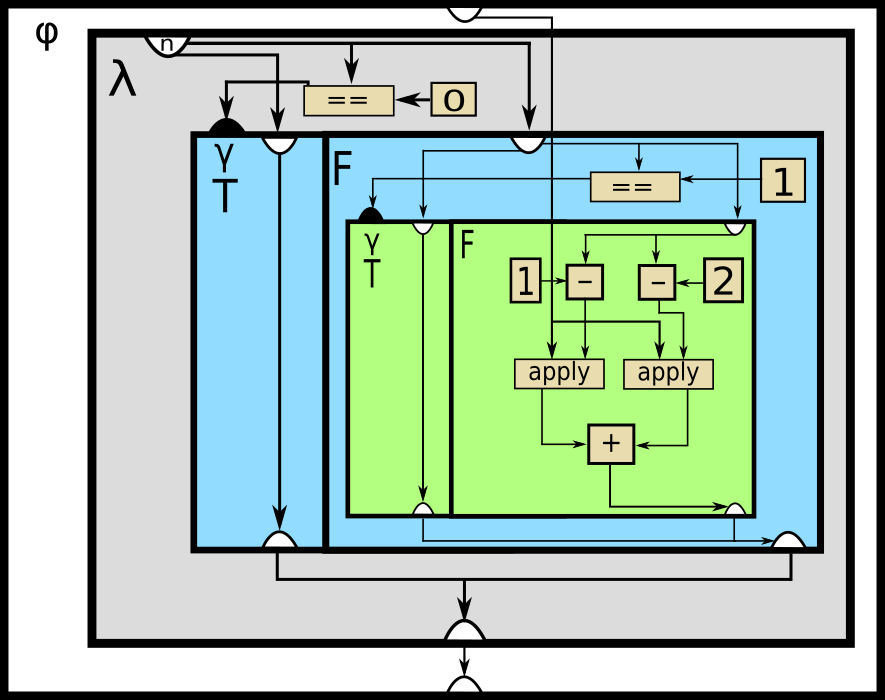
\includegraphics[width=0.75\textwidth]{figures/recursive_fibonacci}
	\caption{A $\phi$-node containing a $\lambda$-node representing a recursive
version of a function producing the $n$ first numbers in the Fibonacci series.}
	\label{fig:rec_fib_phi}
\end{figure}
